\documentclass[a4paper,11pt]{article}

\usepackage[english]{babel}
\usepackage[utf8]{inputenc}
\usepackage[T1]{fontenc}
\usepackage[top=2.5cm,bottom=2.5cm,left=3cm,right=2cm,marginparwidth=1.75cm]{geometry}
\usepackage{setspace}
\usepackage{amsmath}
\usepackage{graphicx}
\usepackage{float}
\usepackage{booktabs}
\usepackage{tabularx}
\usepackage{enumitem}
\usepackage{xcolor}
\usepackage[colorlinks=true, allcolors=blue]{hyperref}
\usepackage[backend=biber,style=authoryear]{biblatex}
\addbibresource{references.bib}

\onehalfspacing
\setlength{\parskip}{0.4em}
\setlength{\parindent}{0pt}
\setlist[itemize]{leftmargin=1.5em}
\setlist[enumerate]{leftmargin=1.7em}

\title{Design and Development of a Hybrid Chatbot for Medical Haematology using Sequential Models for Intent Classification and Retrieval-Based Response Generation}
\author{Student Name: [Insert Name] \\ Student ID: [Insert ID] \\ Programme: [Insert Degree Title] \\ Supervisor: [Insert Supervisor Name]}
\date{May 2026}

\begin{document}
\maketitle

\begin{abstract}
This dissertation presented the design, implementation, testing, deployment, and evaluation of a hybrid medical haematology chatbot built around an explicit MLOps lifecycle. The project addressed a practical gap between general-purpose conversational systems and the narrowly defined needs of haematology laboratory support. General chatbots may provide broad language coverage, but they do not naturally satisfy laboratory requirements for controlled scope, reproducible behaviour, auditability, safe handling of out-of-scope prompts, or continuous operational monitoring. In response to that problem, a domain-specific assistant was developed for English-language haematology workflows, coagulation specimen handling, complete blood count terminology, blood smear support, quality control topics, and report-reading assistance.

The implemented system combined two BiLSTM sequential intent classifiers with retrieval-based response generation, entity-assisted routing, safety rules, PostgreSQL logging, an administrative monitoring panel, and a retraining workflow. A dual-model design was adopted. The first model supported general haematology assistant functions, including workflow and communication intents. The second model targeted blood-report questions, such as CBC parameters, abnormal flags, and report-structure explanations. This design allowed narrower label spaces, targeted monitoring, and model switching when a user query matched the alternative scope more closely.

A fixed 70/15/15 train-validation-test split policy was introduced to strengthen evaluation discipline and reduce leakage between model selection and final reporting. At the time of the final documented evaluation, the master labelled dataset contained 5,391 utterances across 29 intents. The derived general dataset contained 2,670 utterances across 21 intents, and the report dataset contained 4,777 utterances across 26 intents. The general model achieved 0.8928 test accuracy and 0.8649 macro F1, while the report model achieved 0.9358 test accuracy and 0.8965 macro F1 after the report-analysis expansions. In addition, 52 automated tests passed across API, preprocessing, routing, model advisory, split generation, report analysis, and deployment utilities.

It was concluded that the project met its aim of producing a substantial and operational artefact that connected sequential NLP modelling with retrieval-based response generation, report-value information extraction, and practical MLOps controls. The main strengths of the work were controlled deployment scope, reproducible data handling, traceable inference, bounded report analysis, and maintainable operational monitoring. The main limitations were the use of a moderate-sized labelled dataset, English-only support, the absence of patient-specific clinical interpretation, and continued reliance on rule-based entity refinement and reference logic. Nevertheless, the project demonstrated that a hybrid sequential architecture remained appropriate for a bounded medical assistant when supported by disciplined data management, monitoring, and retraining processes.

\end{abstract}

\section{Introduction}
\label{sec:introduction}
\subsection{Background to the Project}

Conversational systems have been adopted widely across healthcare, education, commerce, and customer support. In healthcare, such systems have been used for education, triage support, adherence reminders, self-management, service navigation, and patient communication. However, the literature has shown that many healthcare conversational agents remain limited in evaluation maturity, safety evidence, and usability standardisation (Milne-Ives \textit{et al.}, 2020; Denecke and May, 2022). The problem becomes more acute when the system is expected to operate in a technical environment such as a haematology laboratory, where terminology is specialised and responses must remain controlled.

The project was therefore framed around a narrower and more defensible use case: a medical haematology assistant for laboratory-oriented questions. The purpose was not to produce an autonomous diagnostic system or a treatment recommendation engine. Instead, the aim was to support users with explanations of complete blood count terminology, specimen collection guidance, coagulation sample handling, blood smear concepts, quality control questions, report-structure explanations, and controlled fallback behaviour. This bounded scope was important because the clinical consequences of hallucinated or overly broad medical advice would have been unacceptable.

The project also had an engineering motivation. In many student machine learning projects, most effort is concentrated on the model itself, while the operational lifecycle is treated as an afterthought. That approach is not sufficient for production-style machine learning. Sculley \textit{et al.} (2015) argued that machine learning systems accumulate technical debt through data dependencies, hidden feedback loops, configuration complexity, and fragile system boundaries. Kreuzberger, Kühl and Hirschl (2023) similarly described MLOps as an end-to-end discipline involving data, model, deployment, monitoring, feedback, and retraining. For that reason, this project was defined not only as a chatbot implementation but also as an MLOps-oriented system.

\subsection{Problem Statement}

It was identified that a general-purpose chatbot would not be appropriate for this laboratory-focused scenario for four main reasons. First, general chatbots do not guarantee intent-level control over specialist terminology and laboratory workflows. Second, their outputs are not naturally limited to a safe operational scope. Third, model behaviour cannot be improved systematically unless user queries, low-confidence predictions, and review outcomes are logged and analysed. Fourth, the absence of reproducible train-validation-test separation weakens the credibility of model evaluation.

The project problem was therefore defined as follows: \textbf{how could a domain-specific haematology assistant be designed using sequential intent classification and retrieval-based response generation, while also supporting versioned data, fixed evaluation splits, deployment logging, model monitoring, and retraining from reviewed user queries?}

\subsection{Aim and Objectives}

The overall aim of the project was to design and develop a hybrid chatbot for medical haematology that used sequential models for intent classification and retrieval-based response generation, supported by a practical MLOps workflow.

To achieve that aim, the following objectives were pursued:

\begin{enumerate}

\item A labelled dataset of haematology and operational utterances was to be created and extended iteratively.

\item Sequential intent classifiers based on BiLSTM were to be trained for at least two task scopes.

\item A retrieval-based response layer was to be implemented using curated haematology knowledge rather than unrestricted generation.

\item Safety rules, model switching, and entity-based routing were to be introduced so that the assistant remained within an appropriate scope.

\item A deployable application stack was to be built with API, browser UI, PostgreSQL logging, and Docker support.

\item The machine learning lifecycle was to be formalised through fixed dataset splits, reproducible evaluation, automated testing, monitoring, and retraining support.

\end{enumerate}

\subsection{Research Relevance and Contribution}

The project was relevant to the programme outcomes in three ways. First, it required critical understanding of medical chatbots, sequential neural architectures, retrieval methods, and MLOps principles. Second, it resulted in a substantial technical artefact rather than a purely theoretical study. Third, it demanded evaluation, iteration, and critical reflection on model boundaries, data quality, and operational maintainability.

The specific contribution of the project was not a novel neural architecture. Instead, the contribution lay in the integration of multiple layers into a coherent and auditable system: domain-specific data collection, BiLSTM intent classification, TF-IDF retrieval, model-aware routing, traceable admin diagnostics, retraining from reviewed logs, and split-aware evaluation. In that respect, the work addressed both machine learning and software engineering concerns.

\subsection{Scope and Delimitations}

The scope was intentionally limited. The assistant supported English-language text input only. It was designed to answer laboratory-oriented and report-support questions, not to diagnose disease, prescribe medication, or interpret full patient cases. The system did not attempt multimodal vision analysis of uploaded blood reports, even though report-oriented textual support was provided. Furthermore, the retrieval layer was curated and bounded by a knowledge base, which meant the system could not answer arbitrary medical questions outside the modelled domain.

These delimitations were not weaknesses of planning; they were design decisions taken to maintain a safe and defensible project boundary.


\section{Literature Review}
\label{sec:literature-review}
\subsection{Conversational Agents in Healthcare}

Conversational agents in healthcare have been studied as tools for service support, patient education, coaching, triage, monitoring, and behavioural interventions. Tudor Car \textit{et al.} (2020) reported that the healthcare chatbot literature remained diverse in purpose and format, but often lacked robust evidence for safety, effectiveness, and acceptability. They also observed that many systems were text-based, AI-driven, and mobile or web delivered, which aligned with the deployment assumptions of the present project.

Milne-Ives \textit{et al.} (2020) reviewed the effectiveness of AI conversational agents in healthcare and found encouraging use across multiple tasks, but also highlighted methodological variation and the need for stronger evaluation. Denecke and May (2022) focused specifically on usability assessment and concluded that no standardised procedure yet existed for evaluating healthcare conversational agents. This was important for the current project because it suggested that usability and operational traceability should be documented explicitly rather than assumed.

A recurring conclusion in the literature was that conversational agents should support rather than replace healthcare professionals (Tudor Car \textit{et al.}, 2020). That conclusion directly informed the scope of the chatbot developed here. The project therefore avoided any claim that the system could act as a clinician. Instead, it was positioned as a bounded laboratory assistant with controlled informational output.

\subsection{Sequential Models for Intent Classification}

Intent classification in text-based systems is a supervised sequence classification problem. The order of tokens matters because meaning depends on context, phrase structure, and local dependencies. Recurrent neural networks were developed to model sequential data, but classic RNNs suffered from vanishing and exploding gradients over longer sequences. Long Short-Term Memory was introduced to address that problem through gated memory cells capable of preserving relevant state over time (Hochreiter and Schmidhuber, 1997).

Bidirectional LSTM extended this idea by processing the sequence in forward and backward directions, thereby allowing the representation at a given position to incorporate both left and right context. Graves and Schmidhuber (2005) demonstrated that bidirectional LSTM was effective in sequence tasks where contextual information was crucial. Although the cited work addressed phoneme classification rather than text intent classification, the architectural principle remained relevant: bidirectional processing is useful where interpretation depends on surrounding terms.

The project deliberately chose BiLSTM rather than a transformer-based encoder. That decision was taken for practical and methodological reasons. The available dataset was modest rather than large scale; the deployment target required efficient local inference; and the final-year project title explicitly foregrounded sequential models. In addition, a sequential model with explicit vocabulary, token IDs, and fixed padding made the inference pipeline easier to inspect in the admin trace interface. This supported the educational and evaluative aims of the project.

The limitation of this choice was also acknowledged. Transformer models typically generalise more effectively across varied semantic phrasing when substantial pretraining is available. Consequently, the sequential model required more careful intent boundary design, broader paraphrase coverage, and a stronger data expansion process.

At the NLP pipeline level, sequential modelling was only one part of the design. The implemented system also used rule-based preprocessing, lexical tokenisation, vocabulary encoding, lightweight language detection, rule-based intent short-circuiting for safety or conversational cases, domain-specific entity detection, and later-stage information extraction for report values. This distinction was important for the dissertation because it showed that the artefact was not a pure end-to-end neural chatbot. Instead, it was a layered NLP system in which each technique solved a specific part of the problem.

\subsection{Retrieval-Based Response Generation}

Response generation in task-specific medical assistants can be approached in several ways: hand-written responses, rule-based templates, generative neural models, or retrieval-based methods. A purely rule-based chatbot often becomes brittle because language variation rapidly exceeds manually encoded patterns. A free-text generative model may be more flexible, but the medical domain introduces safety risks, reduced controllability, and greater difficulty in validating responses.

For that reason, a retrieval-based strategy was adopted. The assistant first determined what kind of question had been asked, then selected an answer from a curated knowledge base. This approach aligned with information retrieval principles that treat documents or question-answer entries as weighted term vectors. Salton and Buckley (1988) showed that term-weighting schemes based on weighted single terms were highly effective for automatic text retrieval. In the present system, TF-IDF retrieval was used because it was simple, interpretable, efficient on small corpora, and compatible with controlled answer sets.

The retrieval-based layer was not designed as a replacement for classification. Instead, it complemented the classifier. The intent model determined the response space, while retrieval selected the most appropriate answer within that space. This division of responsibility was important. When the classifier had already identified a narrow operational intent such as \texttt{sample\_collection} or \texttt{quality\_control}, broad entity overrides were not allowed to replace that intent with generic CBC explanations. This design rule reduced wrong-but-plausible responses.

\subsection{MLOps, Monitoring, and Technical Debt}

MLOps extends DevOps principles into the machine learning lifecycle. Kreuzberger, Kühl and Hirschl (2023) described MLOps as involving principles, workflows, roles, and technical components across data collection, validation, training, deployment, monitoring, and retraining. That view was strongly relevant to this project because the chatbot was not merely trained once and frozen. Instead, it was designed to ingest new labelled phrases, rebuild datasets, regenerate fixed splits, retrain specific model profiles, and redeploy with updated artefacts.

Sculley \textit{et al.} (2015) argued that machine learning systems incur hidden technical debt through entanglement, undeclared consumers, data dependencies, and configuration issues. The present project reflected that warning directly. Separate version-relevant artefacts were maintained for configuration, labelled data, derived datasets, fixed splits, model weights, evaluation runs, and knowledge-base content. The admin panel was then used to expose those artefacts through a practical monitoring interface. That design did not eliminate technical debt entirely, but it reduced the invisibility of system state.

\subsection{Research Gap and Justification}

The literature showed a clear need for healthcare chatbots that were safe, scoped, and evaluable. It also showed that MLOps maturity was important for real-world ML systems. However, there remained a gap between those discussions and small-scale, domain-specific educational projects. Many student chatbot systems demonstrate inference, but do not include data versioning, logging, retraining, evaluation discipline, or operational review tools. Conversely, many MLOps examples assume large cloud platforms and do not focus on a bounded medical assistant.

The present project therefore occupied a useful middle ground. It did not claim clinical-scale innovation. Instead, it implemented a realistic and inspectable architecture that connected sequential NLP, retrieval-based generation, deployment controls, and review-driven retraining within a manageable final-year project scope.


\section{Design and Development}
\label{sec:design-development}
\subsection{Development Methodology and SDLC Approach}

An incremental SDLC approach with agile characteristics was adopted. The project did not follow a strict waterfall model because intent labels, routing rules, UI requirements, and monitoring needs changed during implementation. However, the work remained structured through a repeating cycle of requirement clarification, implementation, test execution, issue logging, correction, and documentation.

This approach was reflected in the issue log maintained during development. Problems such as incorrect route priority, stale asset loading, model-selection edge cases, and missing admin diagnostics were recorded and then addressed in subsequent iterations. From an SDLC perspective, the project therefore moved through the classic stages of requirements analysis, design, implementation, testing, deployment, and maintenance, but with feedback loops between them rather than one strictly linear pass.

\subsection{Requirements and Functional Decomposition}

The project requirements were divided into five main capability groups.

First, a machine learning layer was required to classify user utterances into haematology-relevant intents. Second, a response layer was required to deliver safe and relevant answers without relying on unrestricted generation. Third, a web application layer was required to expose the assistant through an accessible chat interface. Fourth, an operational layer was required to record production traffic, flagged phrases, and review decisions. Fifth, a retraining layer was required to convert reviewed user phrases into future training data.

These requirements were then decomposed into concrete modules: data utilities, training pipeline, inference registry, entity detection, retrieval engine, routing engine, API endpoints, browser UI, PostgreSQL store, admin console, review export tools, and retraining scripts.

\begin{figure}[H]
    \centering
    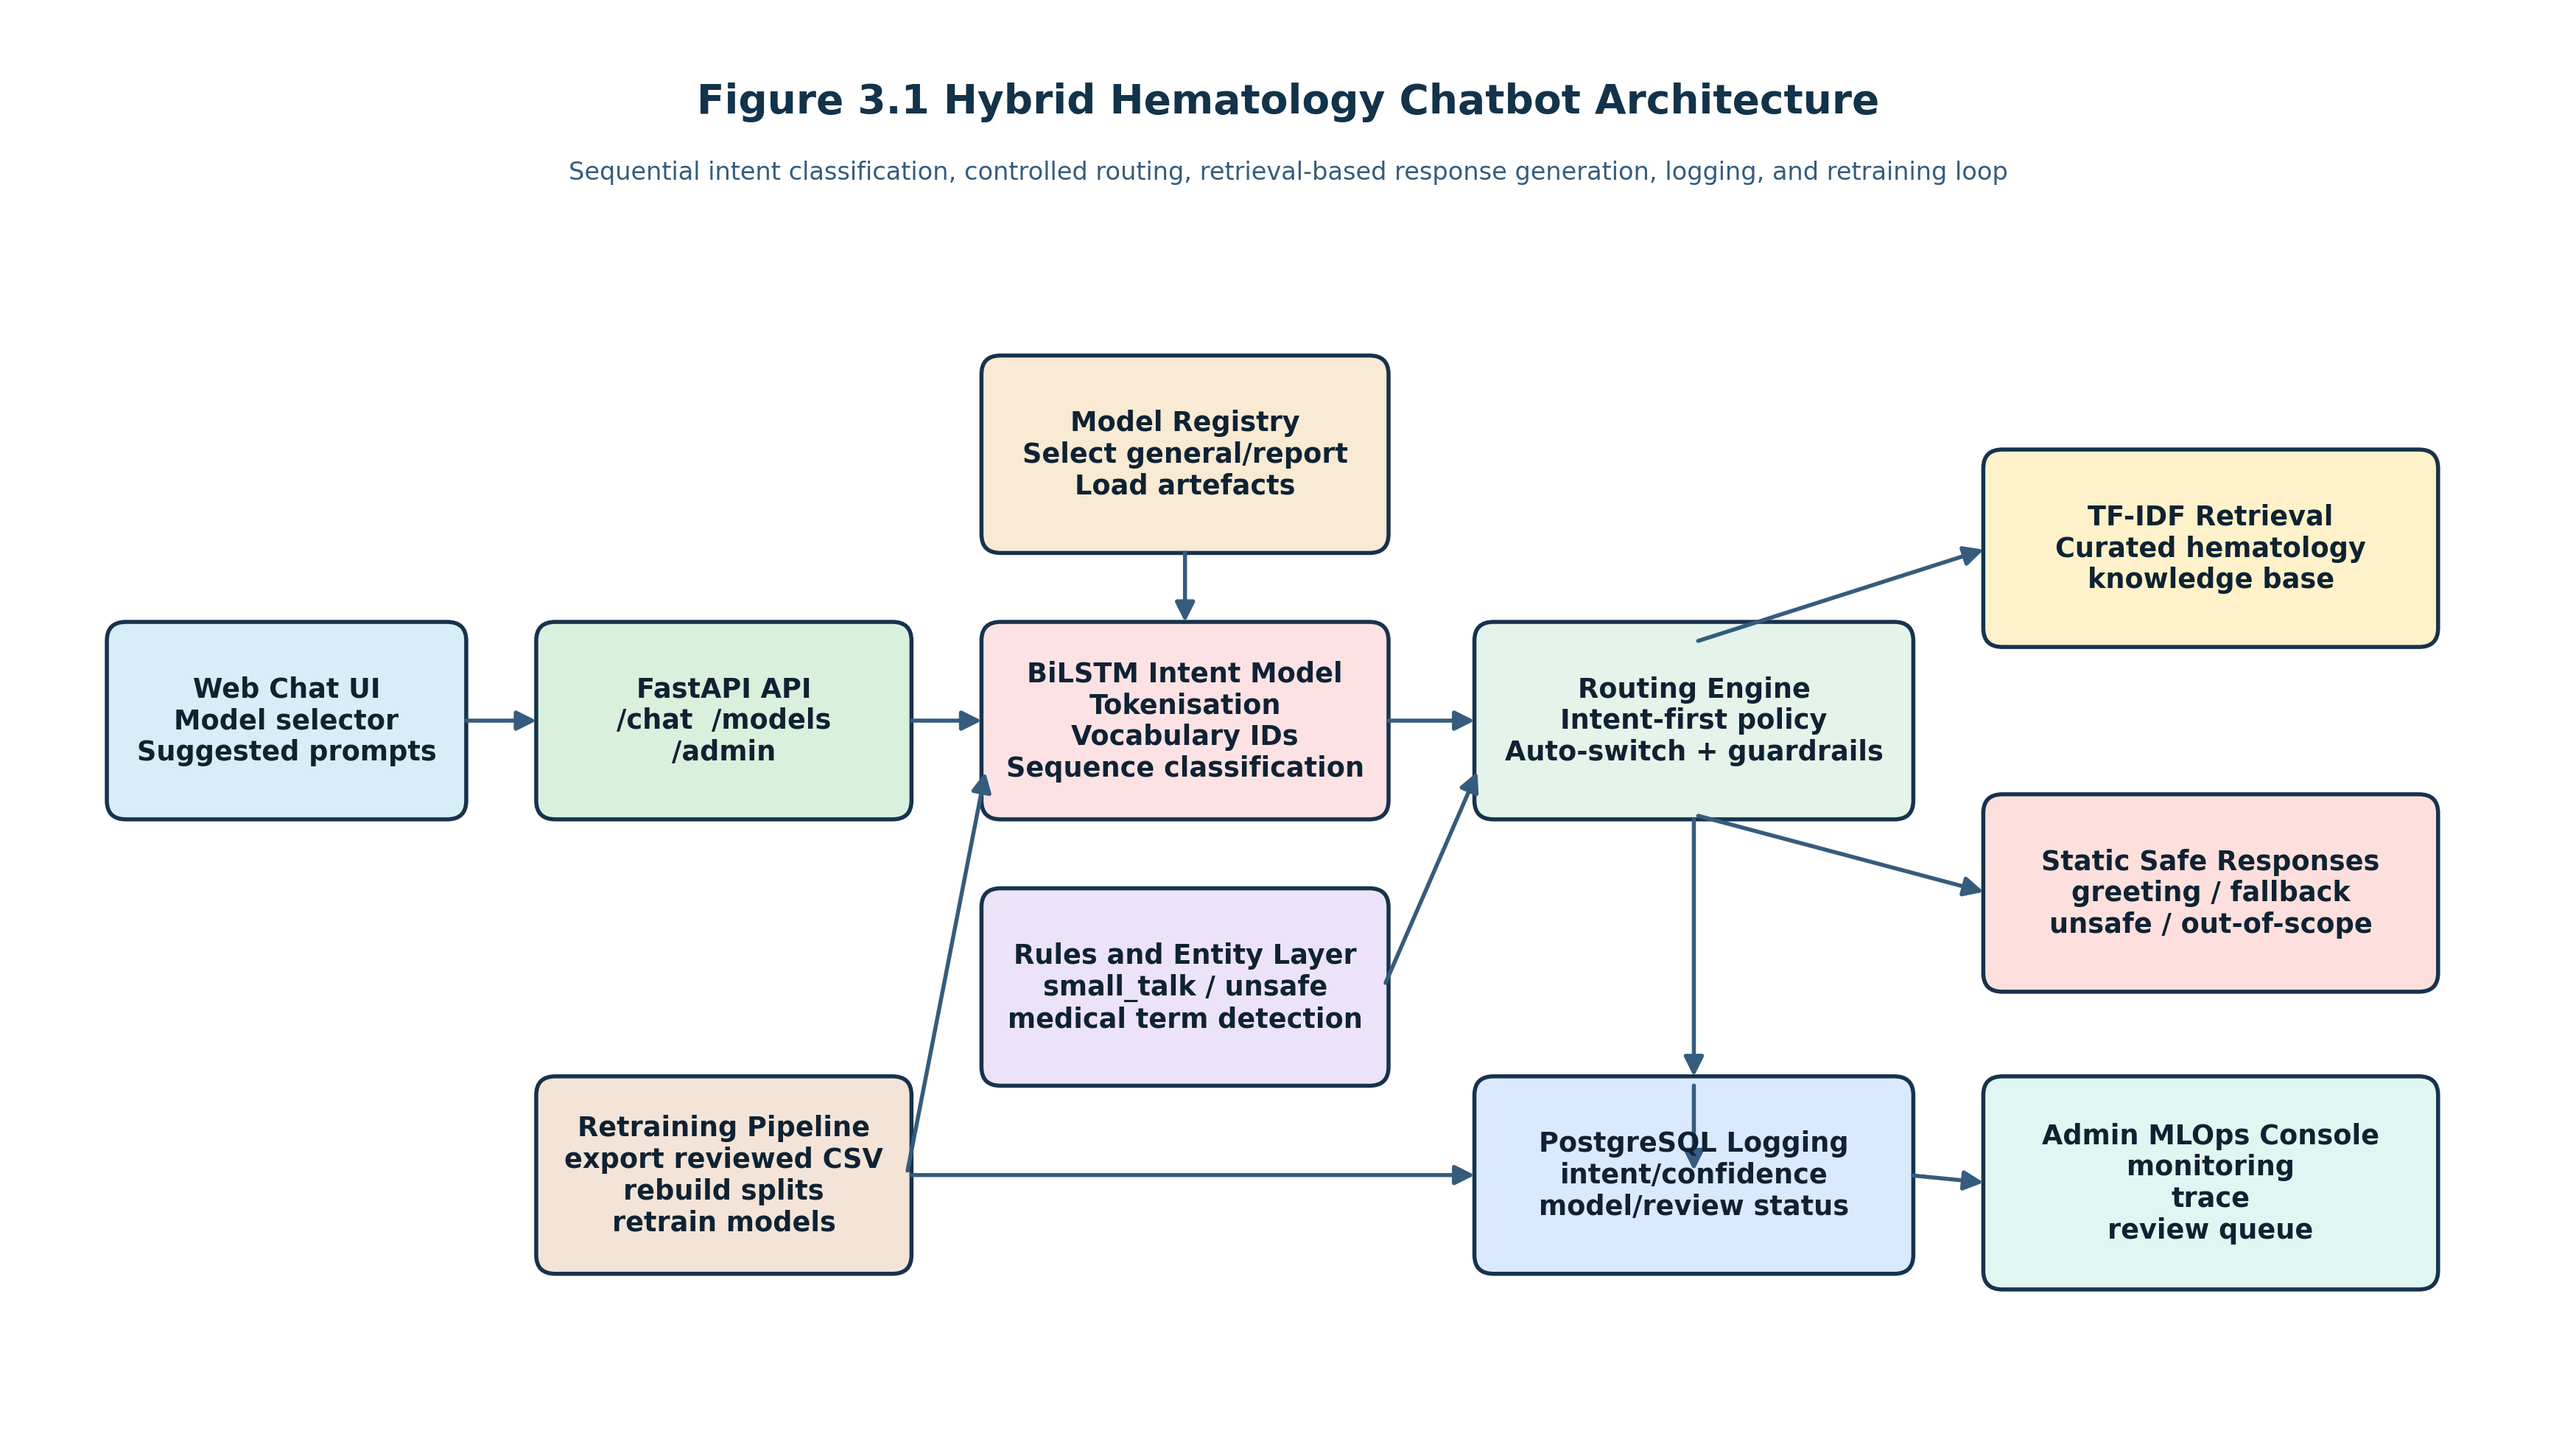
\includegraphics[width=0.9\linewidth]{figures/hybrid_architecture.png}
    \caption{Hybrid haematology chatbot architecture.}
    \label{fig:hybrid-architecture}
\end{figure}

The system was implemented as a hybrid pipeline. A user message was first submitted from the browser UI to a FastAPI backend. A model selector determined whether the \texttt{general} or \texttt{report} profile should be used, with automatic switching when the requested model did not match the detected scope. The selected BiLSTM predictor then normalised the text, tokenised it, converted tokens into vocabulary indices, padded the sequence, and produced intent probabilities. After intent prediction, routing logic decided whether the answer should come from a static control response or the retrieval layer. Entity detection could refine retrieval within broad medical intents, but was constrained from overriding already-specific operational intents.

\subsection{Dataset Design and Growth Strategy}

The dataset strategy was central to the project. Rather than relying on a single fixed file, the data lifecycle was divided into reusable stages. Raw inputs were kept separate from labelled phrase files. A master training dataset was then built from labelled inputs, and model-specific datasets were derived from that master file. Fixed train, validation, and test splits were then generated from the derived datasets.

At the time of final documentation, the master dataset contained 5,391 labelled utterances across 29 intents. The general model dataset contained 2,670 utterances across 21 intents, while the report model dataset contained 4,777 utterances across 26 intents. Large classes included \texttt{cbc\_info=312}, \texttt{coag\_test=300}, \texttt{sample\_collection=214}, and \texttt{report\_numeric\_result\_analysis=1,219}. Additional data was added iteratively to improve weak classes such as \texttt{small\_talk}, \texttt{capability\_query}, \texttt{coag\_test}, and multi-value report-analysis prompts.

The design rationale for two model profiles was straightforward. The \texttt{general} model was intended for workflow, specimen handling, QC, coagulation, smear, and communication intents. The \texttt{report} model was intended for CBC parameter, flag, abnormality, and report-structure support. Some vocabulary overlap was expected because both models operated in the same domain. However, separate datasets reduced label competition between workflow questions and report-reading questions.

\subsection{Preprocessing Pipeline}

Text preprocessing was kept explicit and inspectable. Input text was normalised and tokenised into simple lexical units. A vocabulary was built from the training split, and each token was converted into an integer index. Sequences were then padded to a fixed maximum length so that they could be batched efficiently. A train-validation-test split of 70/15/15 was adopted and fixed on disk for reproducibility. The general split produced 1,868 training rows, 401 validation rows, and 401 test rows. The report split produced 3,343 training rows, 717 validation rows, and 717 test rows after the report-analysis expansions.

This split-aware process was introduced because earlier single-holdout evaluation made it difficult to distinguish model selection from final testing. By separating validation from test, the best checkpoint could be chosen using validation F1 while leaving the test set untouched for final reporting.

\subsection{Sequential Model Design}

The intent classifier was implemented as a BiLSTM with an embedding layer, recurrent sequence encoder, and classification head. The input sequence was embedded into dense vectors, processed bidirectionally, pooled, and then projected to the intent label space. In NLP terms, this stage performed token-sequence modelling over a bounded vocabulary rather than free-text generation. Training used batch size 64, learning rate 0.001, weight decay 1e-05, and 8 epochs in the reported runs.

The general model reached its best validation F1 at epoch 7 with a validation F1 of 0.8978. After the report-analysis and multi-value expansions, the report model also reached its best validation F1 at epoch 7, where validation F1 rose to 0.9444 on the larger report dataset. These results suggested that the models were learning useful structure without severe early overfitting. However, the gap between validation and test performance indicated that the datasets were still moderately challenging and somewhat imbalanced.

\subsection{Retrieval Layer and Knowledge Base}

The knowledge base was stored as curated haematology response entries in JSONL format. Each entry linked an intent and a canonical question to an approved answer. A TF-IDF retrieval layer with unigram and bigram weighting ranked candidate answers against the user utterance and returned the highest-scoring match within the permitted intent scope. Cosine similarity was then used to score the overlap between the user phrase and the curated knowledge entries.

This design had several advantages. First, response text remained controlled and auditable. Second, exact knowledge gaps could be addressed by adding or editing individual entries without retraining the neural model. Third, the retrieval layer could be traced visibly in the admin panel by showing candidate matches and similarity scores. Fourth, the retrieval engine operated within the predicted intent, which reduced the risk of broad but semantically plausible answers crossing into the wrong operational scope.

The main trade-off was that answer quality depended heavily on knowledge-base coverage. If a specific question had not been represented in the curated answer store, the classifier could still be correct while the final answer remained too general. This happened during development with specimen rejection, CBC tube questions, and report-analysis prompts, and was corrected by expanding retrieval entries, introducing a bounded report-analysis layer, and tightening route priority.

\subsection{Safety Rules, Communication Intents, Model Switching, and Report Analysis}

The project implemented dedicated intents for greeting, thanks, goodbye, small talk, clarification, capability questions, incomplete queries, out-of-scope prompts, and unsafe medical requests. This design avoided a common chatbot failure in which non-medical phrases are forced artificially into medical classes. In NLP terms, these intents were handled through a mixture of learned classification and rule-priority short-circuiting so that high-risk phrases did not depend only on the softmax output of the BiLSTM.

A separate model advisory and auto-switch mechanism was also introduced. If a user selected the \texttt{general} model but asked a report-oriented question, the request could be answered by the \texttt{report} model instead. Conversely, if the \texttt{report} model was selected for a workflow question such as specimen tube handling, the system could switch back to the \texttt{general} model. This improved usability without requiring the user to understand the internal architecture.

An additional NLP layer was added for report analysis. Report-like phrases such as \texttt{WBC is 13.7}, \texttt{My report shows anemia}, or \texttt{Age is 50 WBC is 13 MCV is 73 PLT is 1} could not be handled reliably through pure intent classification alone because they required lightweight information extraction after the intent had been recognised. A bounded report-analysis module was therefore implemented to extract analyte labels, numeric values, age, sex markers, and printed report flags. The extracted values were then compared against controlled adult, paediatric, or sex-specific reference intervals. This layer remained rule-bounded and did not perform diagnosis. Its purpose was to support report reading, not clinical decision making.

\begin{figure}[H]
    \centering
    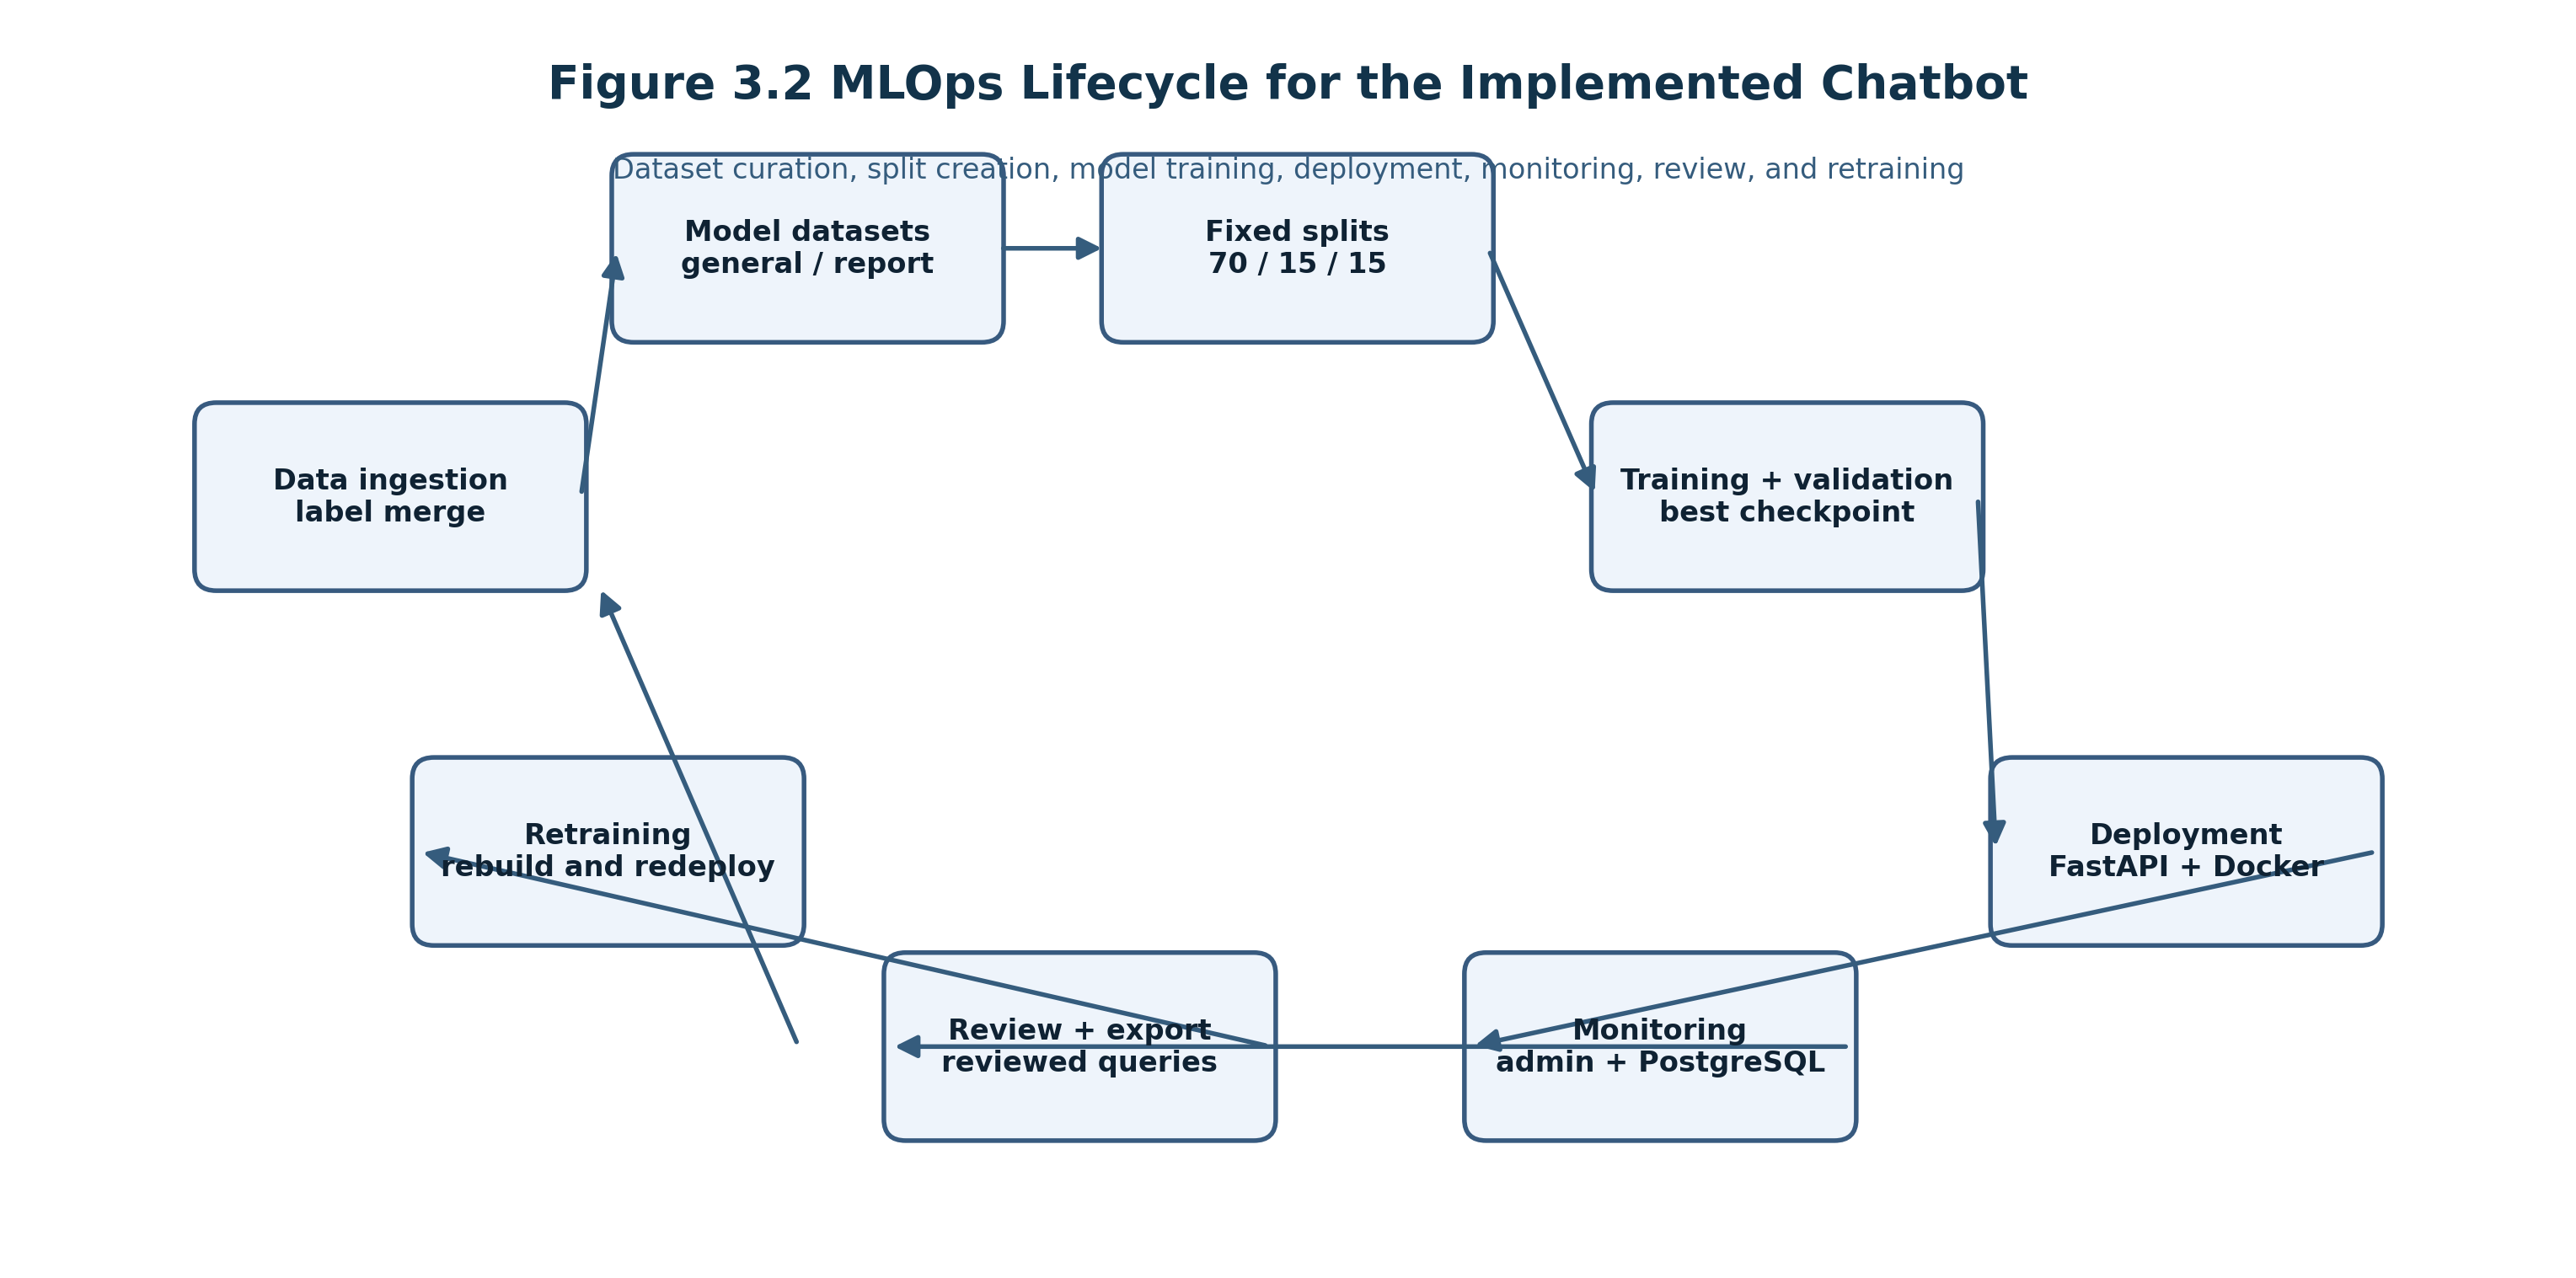
\includegraphics[width=0.88\linewidth]{figures/mlops_lifecycle.png}
    \caption{MLOps lifecycle used in the implemented chatbot project.}
    \label{fig:mlops-lifecycle}
\end{figure}

\begin{figure}[H]
    \centering
    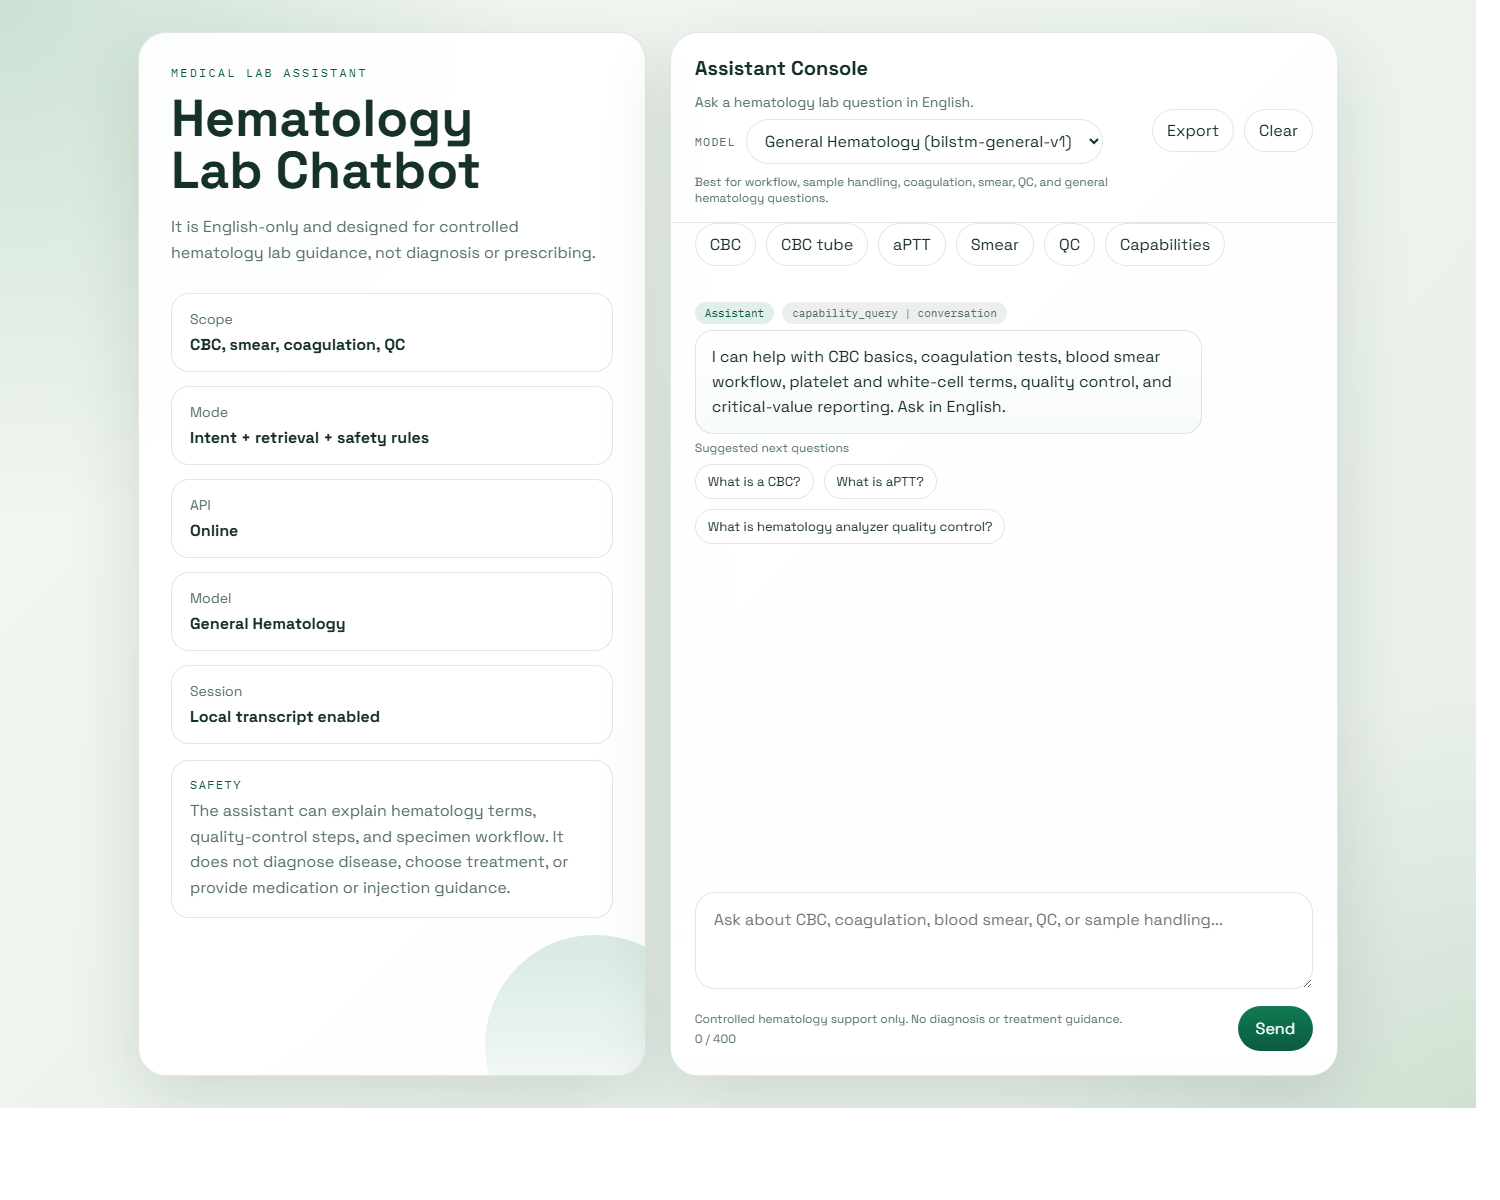
\includegraphics[width=0.74\linewidth]{figures/chat_ui.png}
    \caption{Implemented browser-based chat interface.}
    \label{fig:chat-ui}
\end{figure}

The deployment stack used FastAPI for the HTTP API, PostgreSQL for persistent log storage, static web assets for the chat and admin UIs, and Docker Compose for production-style service composition. The admin console was designed explicitly around MLOps concerns. It included sections for overview metrics, inference trace, data preprocessing, and review queue. Metrics included fallback rate, guardrail rate, low-confidence rate, retrieval rate, and auto-switch rate.

The inference trace view was particularly useful because it exposed the backend path of a single phrase: normalised text, tokens, vocabulary IDs, hard-rule matches, top intent probabilities, entity matches, retrieval candidates, and final routing decision. This feature turned the model from a black box into a partially inspectable system, which was valuable for both debugging and dissertation evidence.

A retraining pipeline was also implemented. Reviewed production phrases could be exported from PostgreSQL into labelled CSV, merged into the master dataset, used to rebuild derived datasets and fixed splits, and then fed back into model training and evaluation. In this way, the project satisfied a core MLOps requirement: feedback from live usage could be converted into future model improvement.


\section{Result Analysis and Evaluation}
\label{sec:results-evaluation}
\subsection{Evaluation Design}

The evaluation strategy combined model metrics, software testing, and operational inspection. For machine learning metrics, fixed train-validation-test splits were used so that the final test set remained isolated from checkpoint selection. For software quality, automated tests covered API behaviour, preprocessing, routing, entity detection, model advisory, inference rules, and split utilities. For operational quality, the admin console and trace tools were used to inspect model behaviour under realistic phrases.

This multi-layer evaluation approach was necessary because the project was hybrid. A high intent accuracy alone would not have proved that final answers were appropriate, nor would a working UI alone have proved that the classifiers were reliable. The evaluation therefore examined the full path from phrase input to logged output.

\begin{table}[H]
    \centering
    \caption{Final held-out test metrics for the two model profiles.}
    \label{tab:final-metrics}
    \begin{tabular}{lccccc}
        \hline
        Model & Accuracy & Macro F1 & Weighted F1 & Macro Precision & Macro Recall \\
        \hline
        General & 0.8928 & 0.8649 & 0.8914 & 0.8822 & 0.8617 \\
        Report & 0.9358 & 0.8965 & 0.9360 & 0.8968 & 0.9040 \\
        \hline
    \end{tabular}
\end{table}

\begin{figure}[H]
    \centering
    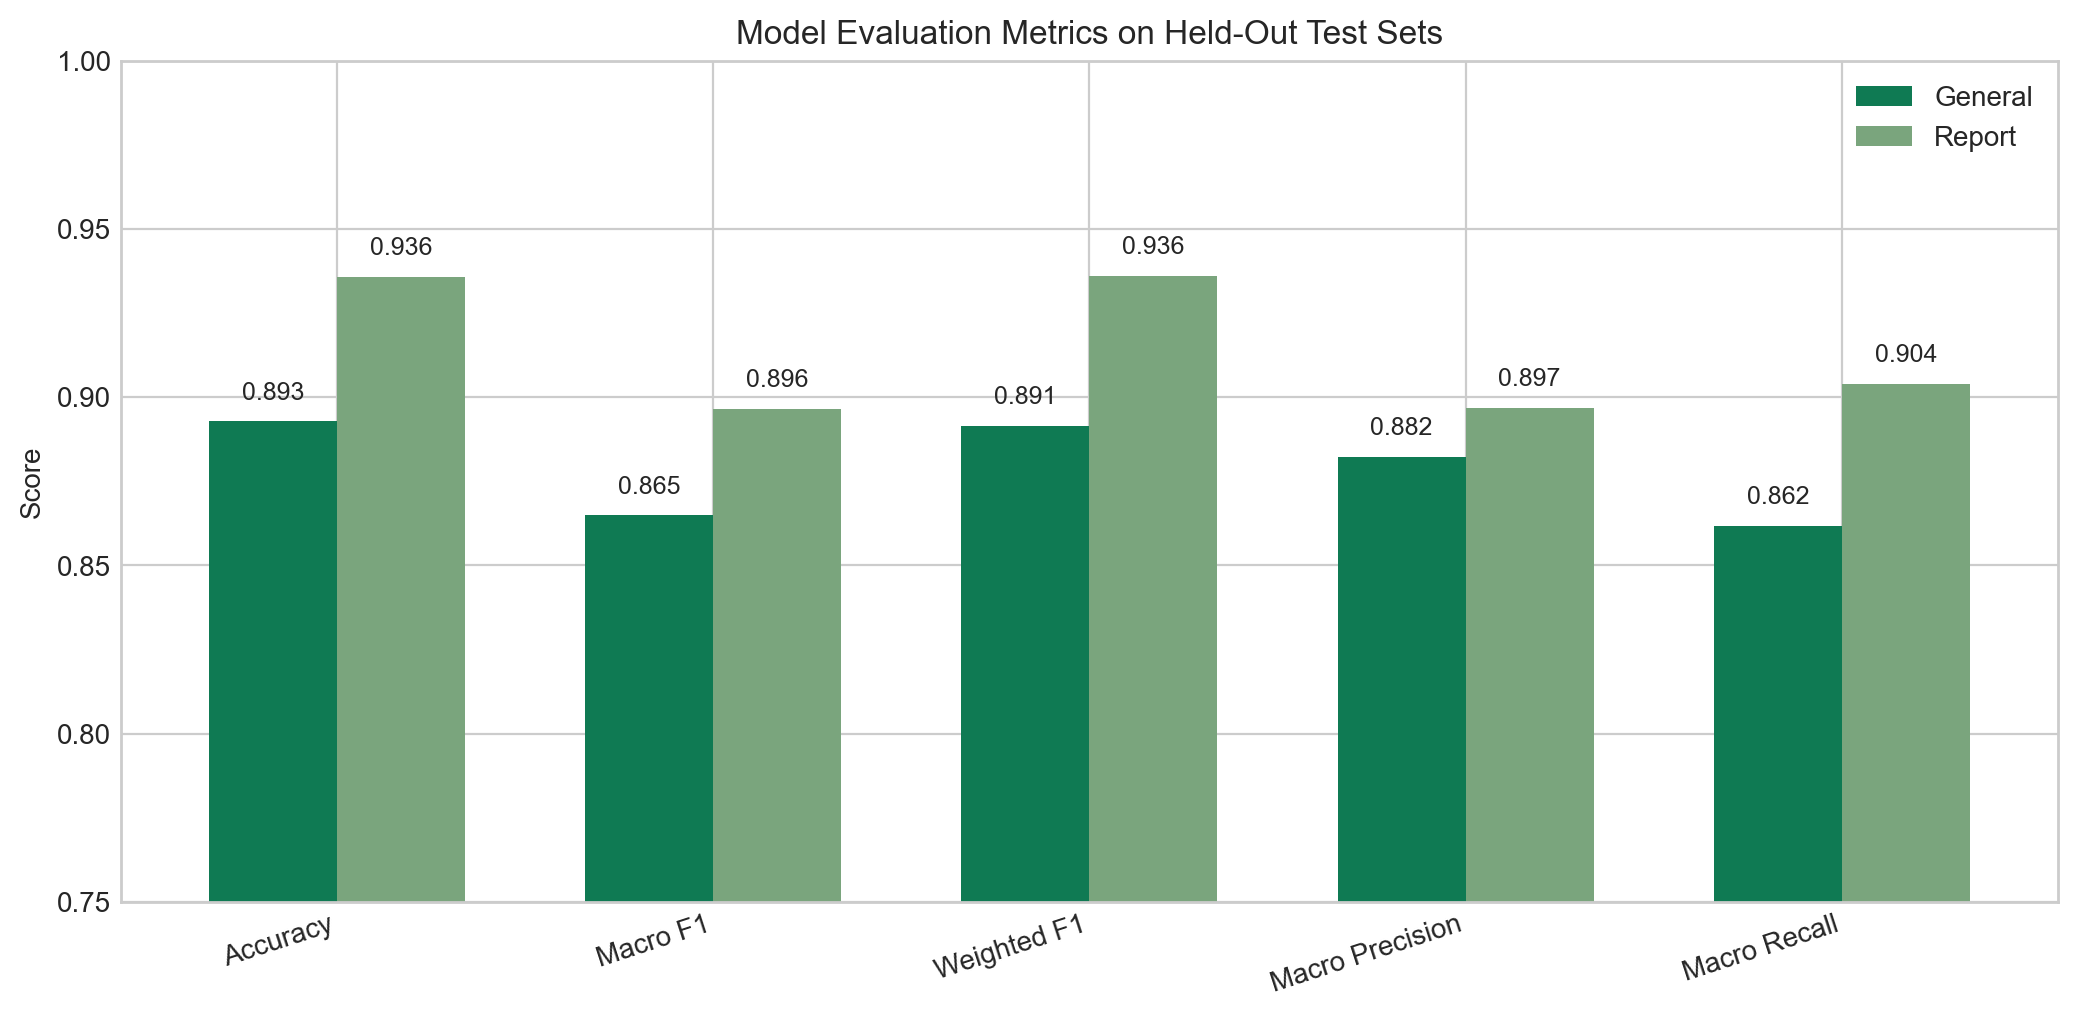
\includegraphics[width=0.88\linewidth]{figures/metric_comparison.png}
    \caption{Metric comparison across the general and report model profiles.}
    \label{fig:metric-comparison}
\end{figure}

\begin{figure}[H]
    \centering
    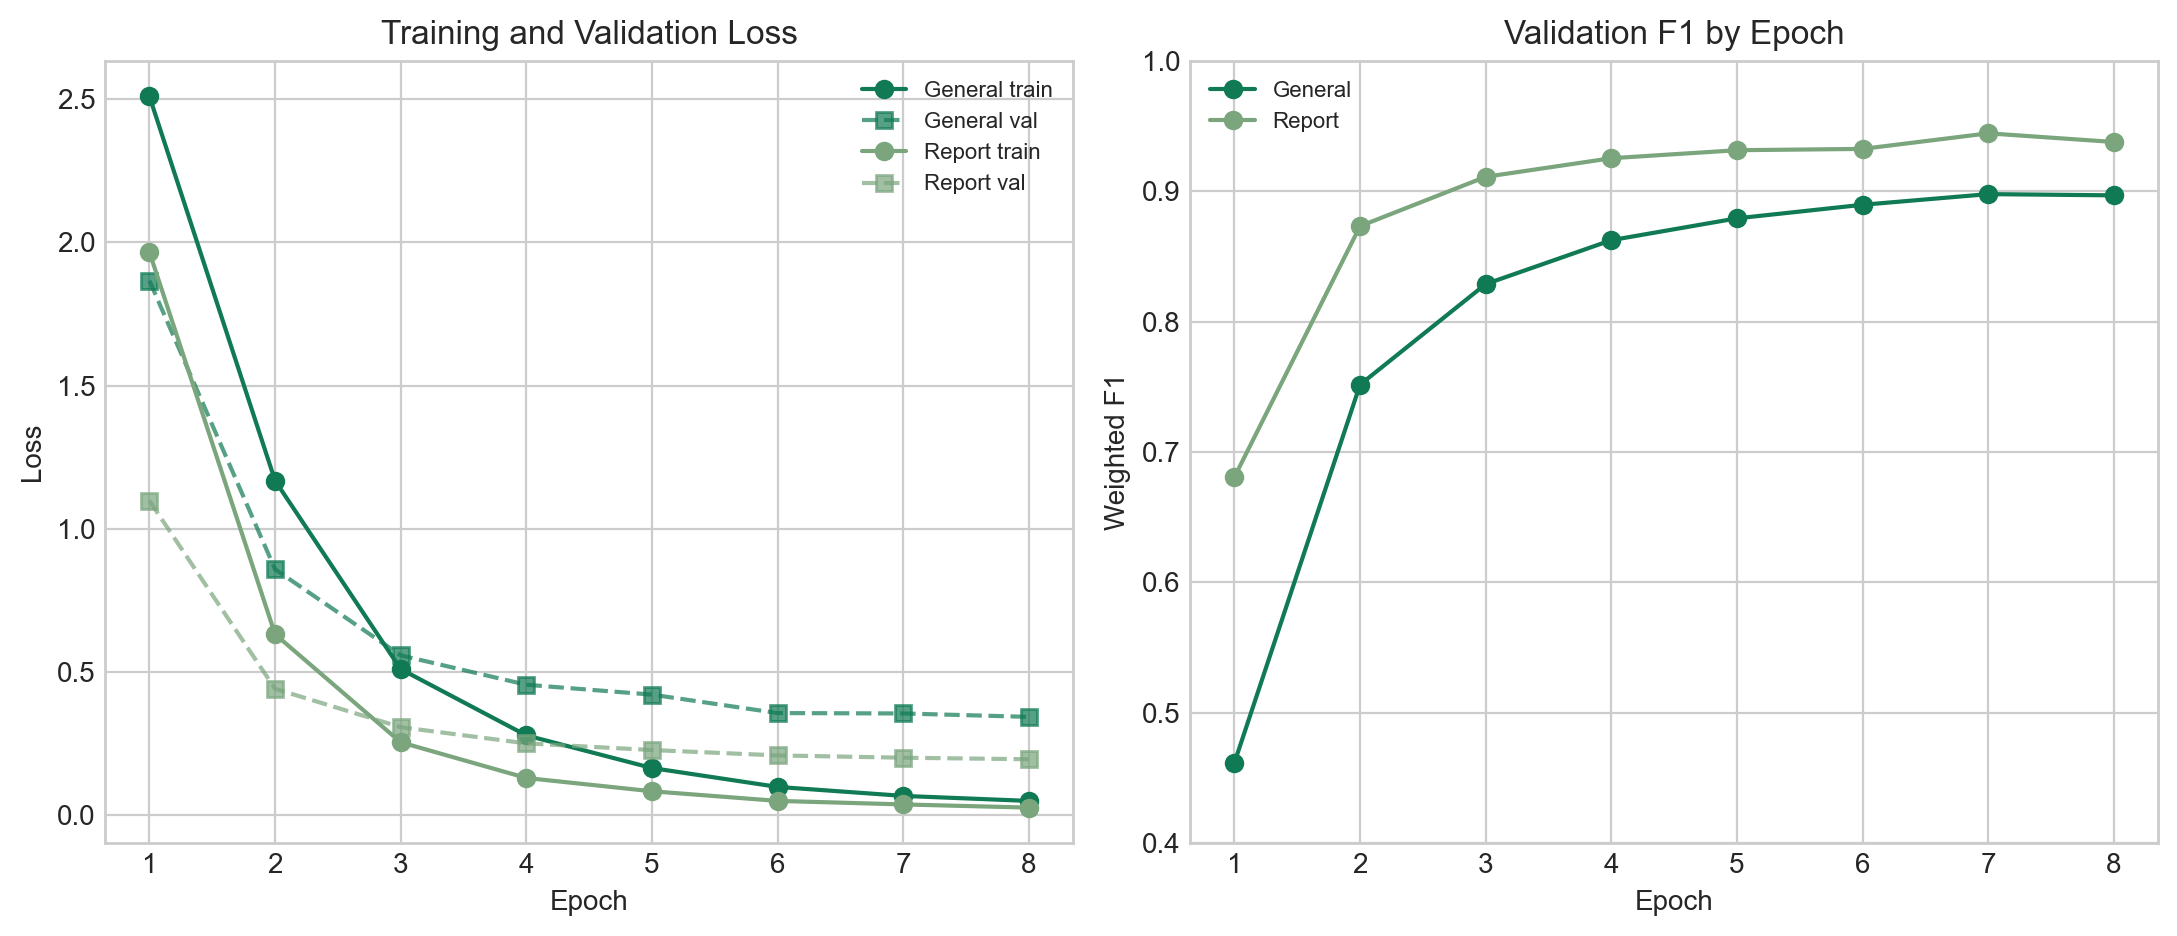
\includegraphics[width=0.88\linewidth]{figures/training_curves.png}
    \caption{Training loss and validation F1 behaviour over the eight-epoch schedule.}
    \label{fig:training-curves}
\end{figure}

\begin{figure}[H]
    \centering
    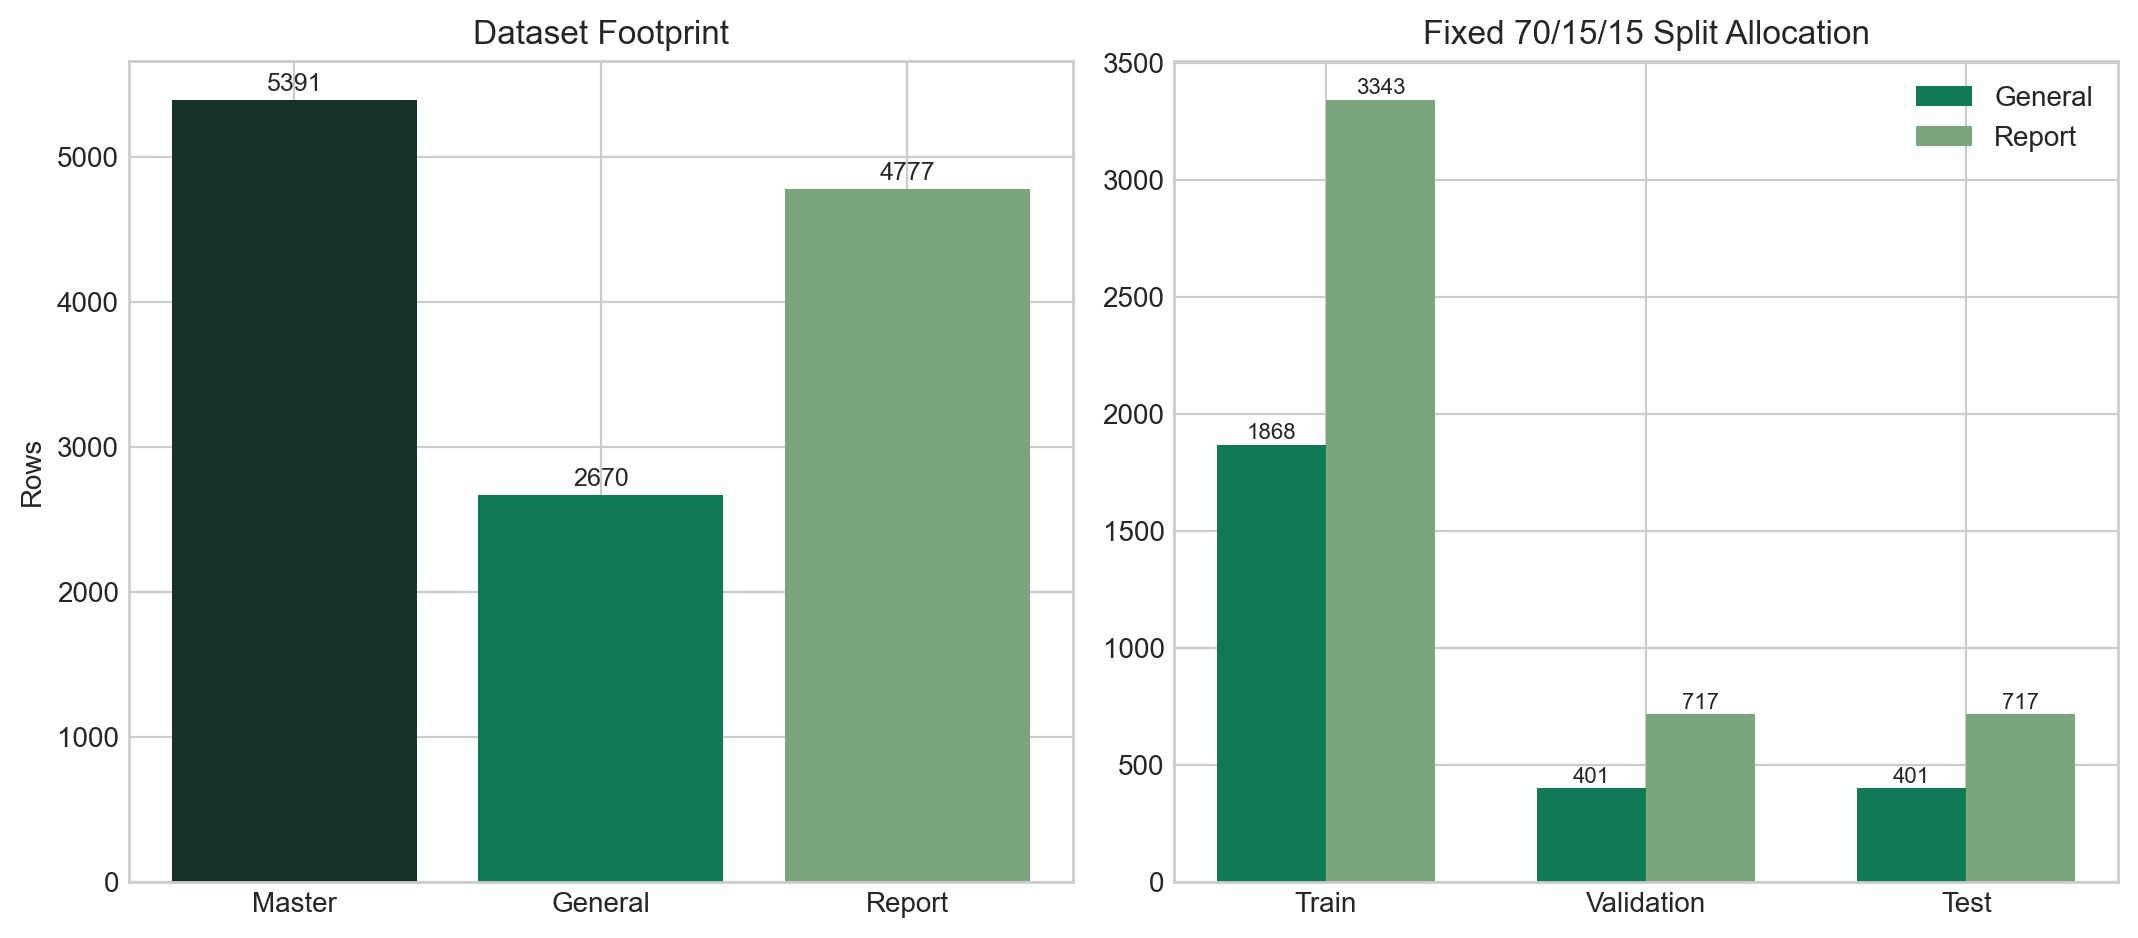
\includegraphics[width=0.88\linewidth]{figures/dataset_splits.png}
    \caption{Dataset footprint and fixed 70/15/15 split allocation.}
    \label{fig:dataset-splits}
\end{figure}

The split-aware evaluation produced more conservative but more defensible results than the earlier single-holdout runs. The general model achieved 0.8928 accuracy, 0.8649 macro F1, 0.8914 weighted F1, 0.8822 macro precision, and 0.8617 macro recall on 401 test examples. The report model achieved 0.9358 accuracy, 0.8965 macro F1, 0.9360 weighted F1, 0.8968 macro precision, and 0.9040 macro recall on 717 test examples after the report-analysis retraining cycle.

These values were strong enough for the scope of the project, especially given the multi-intent label space and safety-oriented conversation classes. The report model achieved higher accuracy after focused data expansion because its report-focused dataset was extended with numeric phrases, printed flags, paediatric phrasing, sex-specific HGB/HCT cases, age-aware prompts, and multi-value report inputs. The general model still faced a broader operational scope, including communication and safety intents, which introduced more heterogeneous phrasing.

\subsection{Training Behaviour, Bias, and Variance Discussion}

The recorded training histories suggested that both models improved steadily over the 8-epoch schedule. For the general model, training loss decreased from 2.5087 to 0.0509 while validation F1 increased from 0.4617 to a best of 0.8978. For the report model, training loss decreased from 1.9654 to 0.0275 while validation F1 increased from 0.6808 to a best of 0.9444. This indicated that the models were not underfitting.

However, the final test macro F1 values of 0.8649 and 0.8965 were lower than the best validation F1 values, which suggested that some generalisation gap remained. That gap was not severe enough to invalidate the models, but it demonstrated that the project could not claim perfect robustness. Several causes were plausible: moderate dataset size, class imbalance, overlap in domain vocabulary, synthetic paraphrase influence, and remaining variation in real conversational phrasing.

It would have been simplistic to describe every output weakness as bias or variance alone. In this project, failure cases also emerged from retrieval coverage gaps, intent overlap, and routing policy. This observation was important because it showed why MLOps evaluation had to go beyond a single classifier score.

\begin{figure}[H]
    \centering
    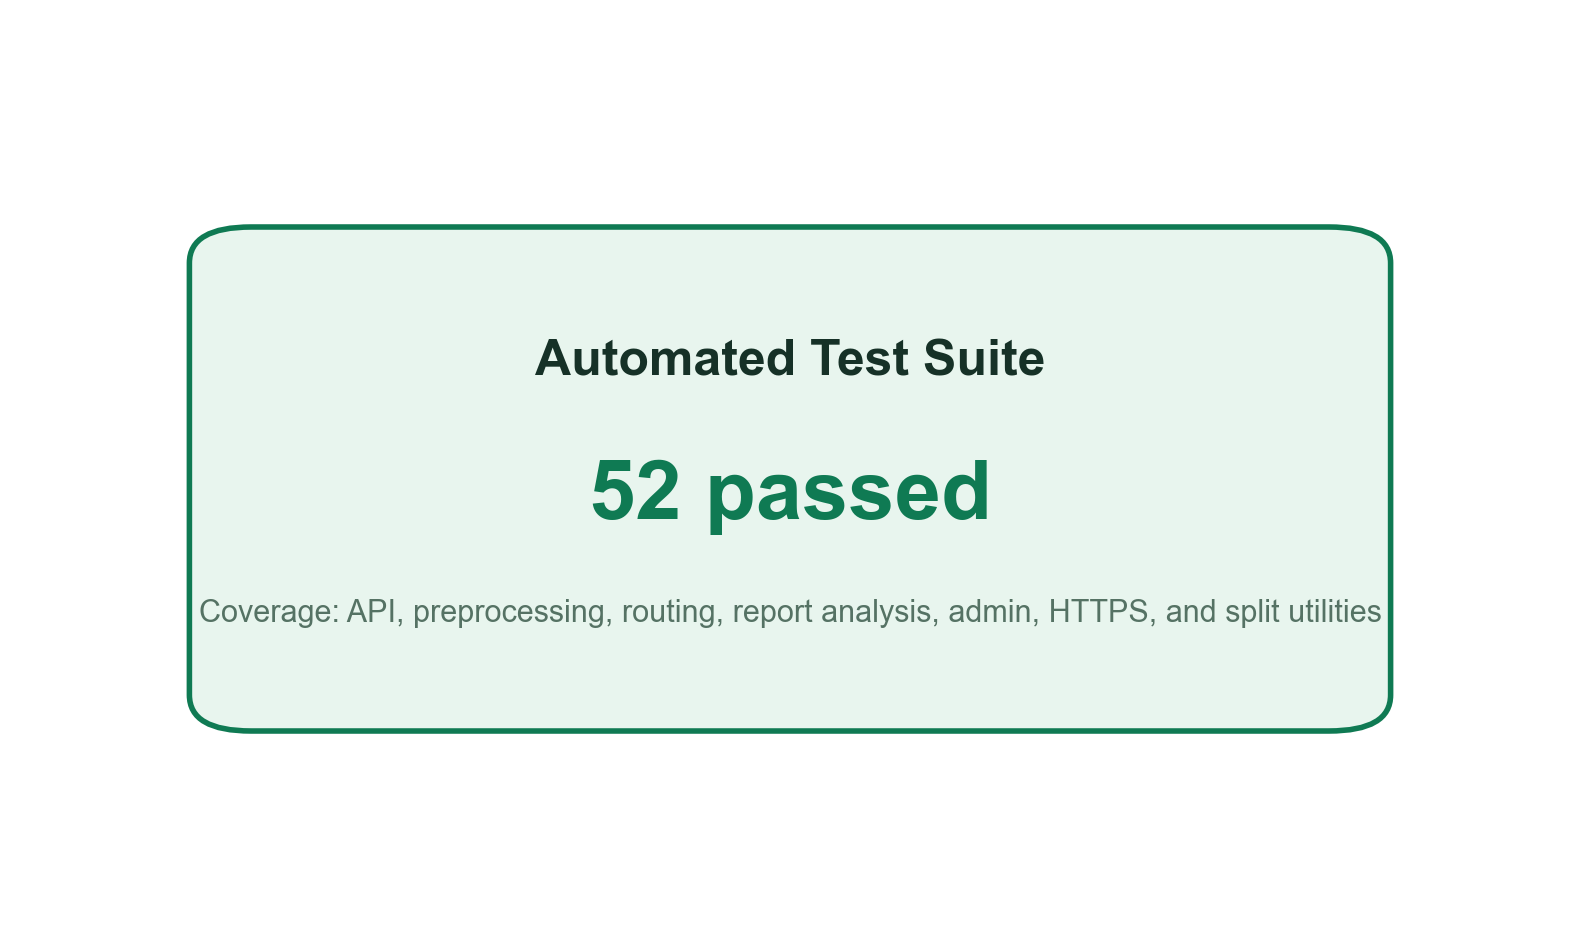
\includegraphics[width=0.72\linewidth]{figures/testing_summary.png}
    \caption{Automated test execution summary showing 52 passing tests.}
    \label{fig:testing-summary}
\end{figure}

At the time of final verification, the full automated test suite passed with 52 tests. These tests covered the major subsystems of the artefact:

\begin{itemize}

\item API endpoint behaviour.

\item Text preprocessing functions.

\item Inference post-processing and fallback handling.

\item Entity detection rules.

\item Routing priorities.

\item Model advisory and auto-switch logic.

\item Predictor rule shortcuts.

\item Report-analysis extraction and interpretation.

\item HTTPS deployment helpers and certificate monitoring.

\item Split generation utilities.

\end{itemize}

This testing strategy aligned with software engineering practice rather than model-only experimentation. It was particularly valuable for regression control. During development, changes to routing and admin features could have introduced silent failures in other areas. The automated suite reduced that risk.

\begin{figure}[H]
    \centering
    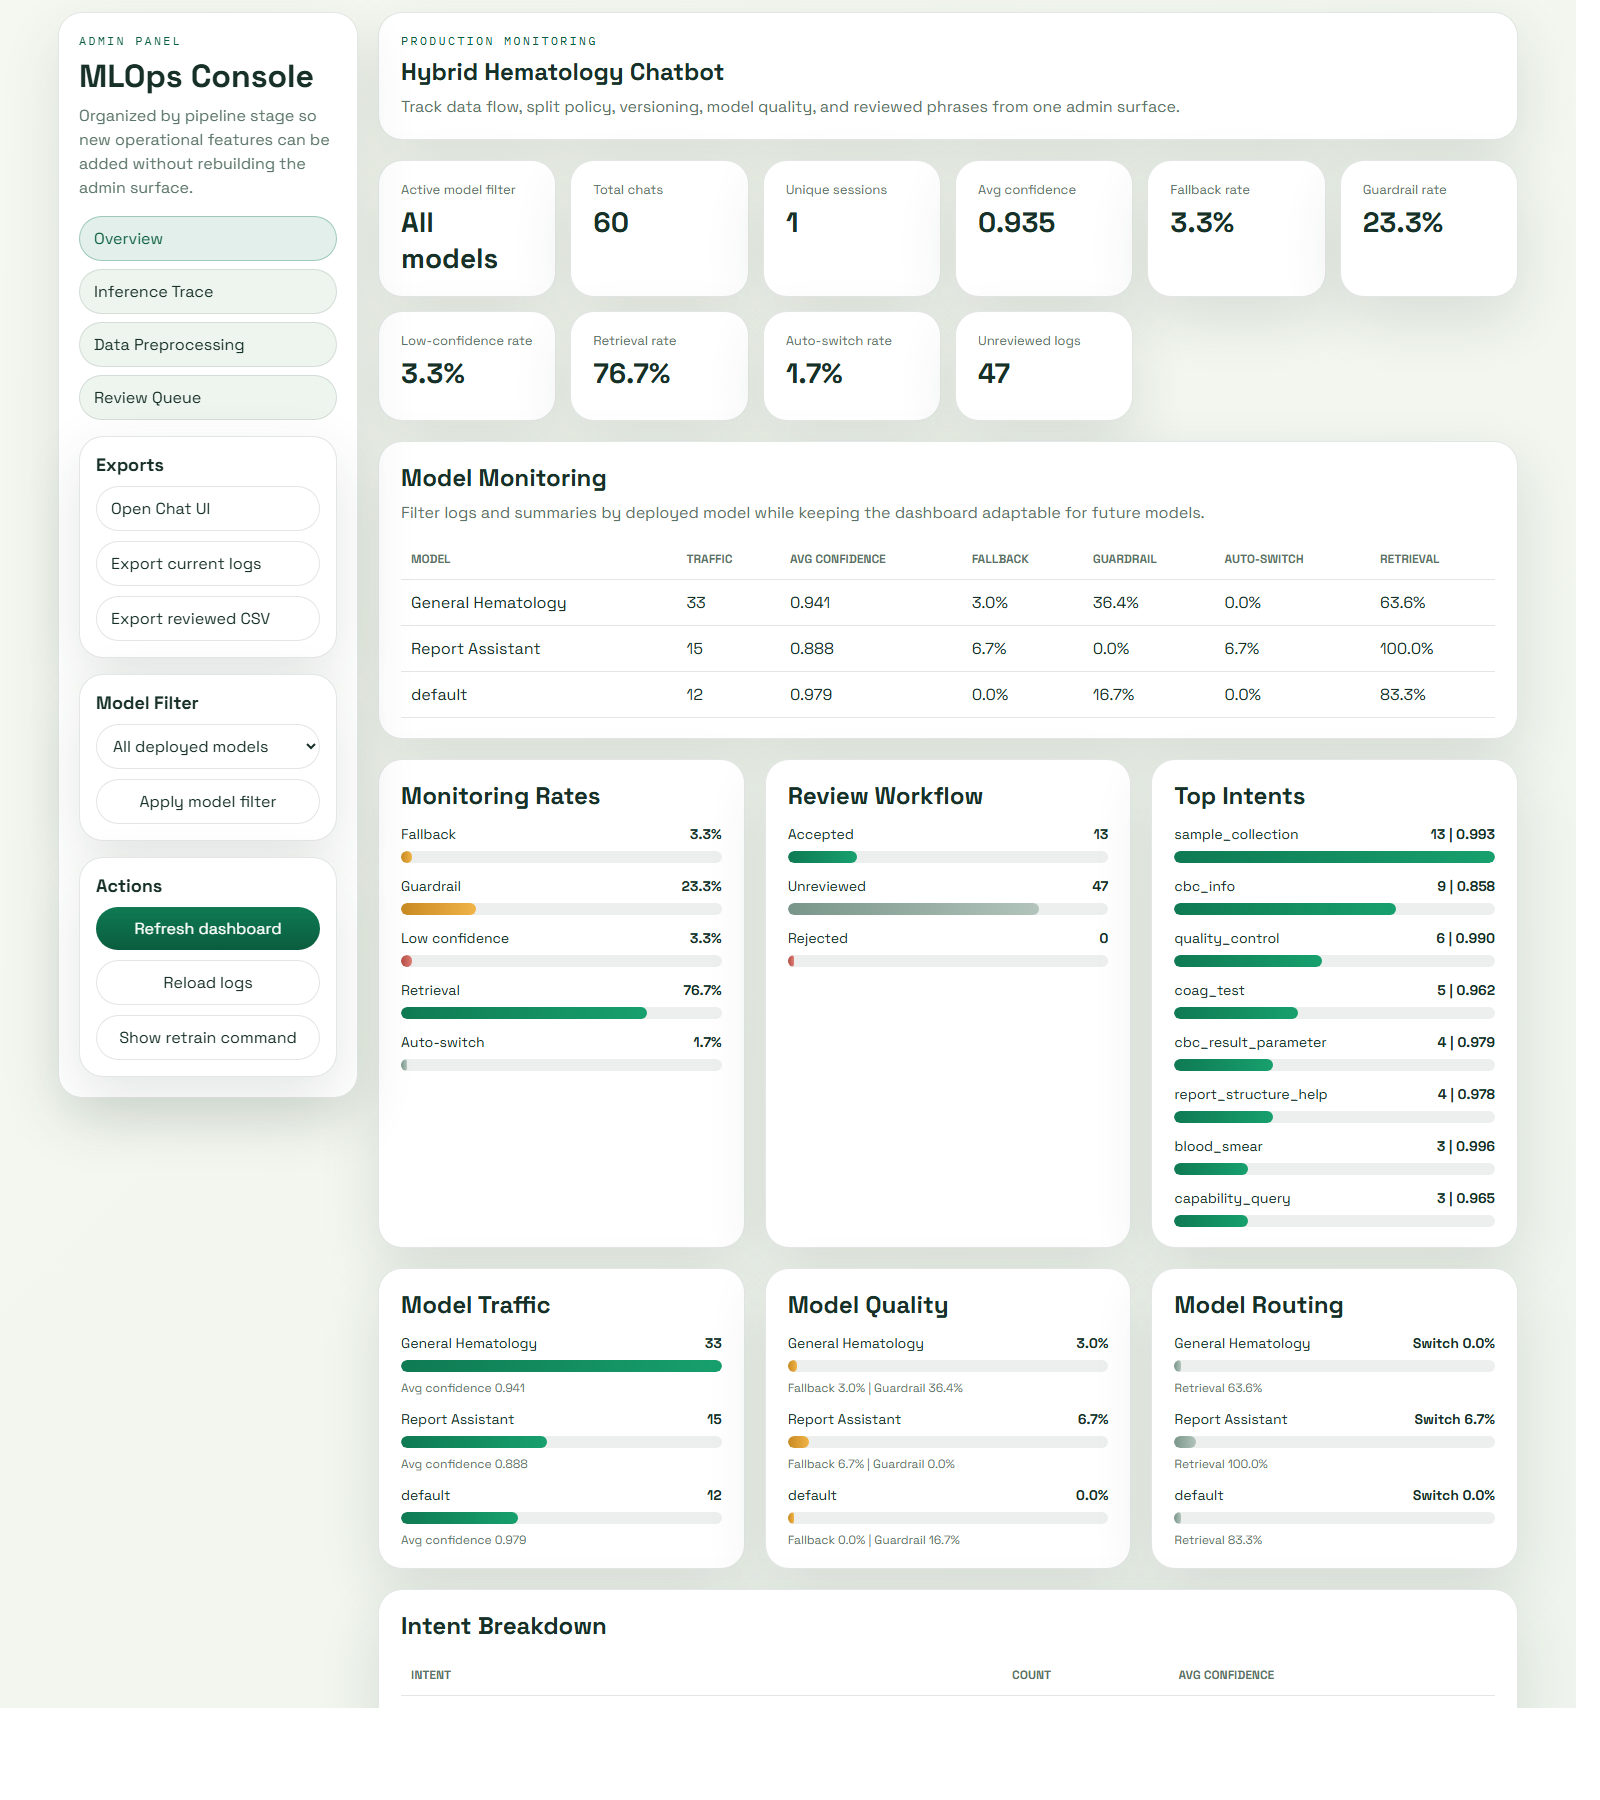
\includegraphics[width=0.88\linewidth]{figures/admin_overview.png}
    \caption{Admin overview dashboard used for operational monitoring and review.}
    \label{fig:admin-overview}
\end{figure}

\begin{figure}[H]
    \centering
    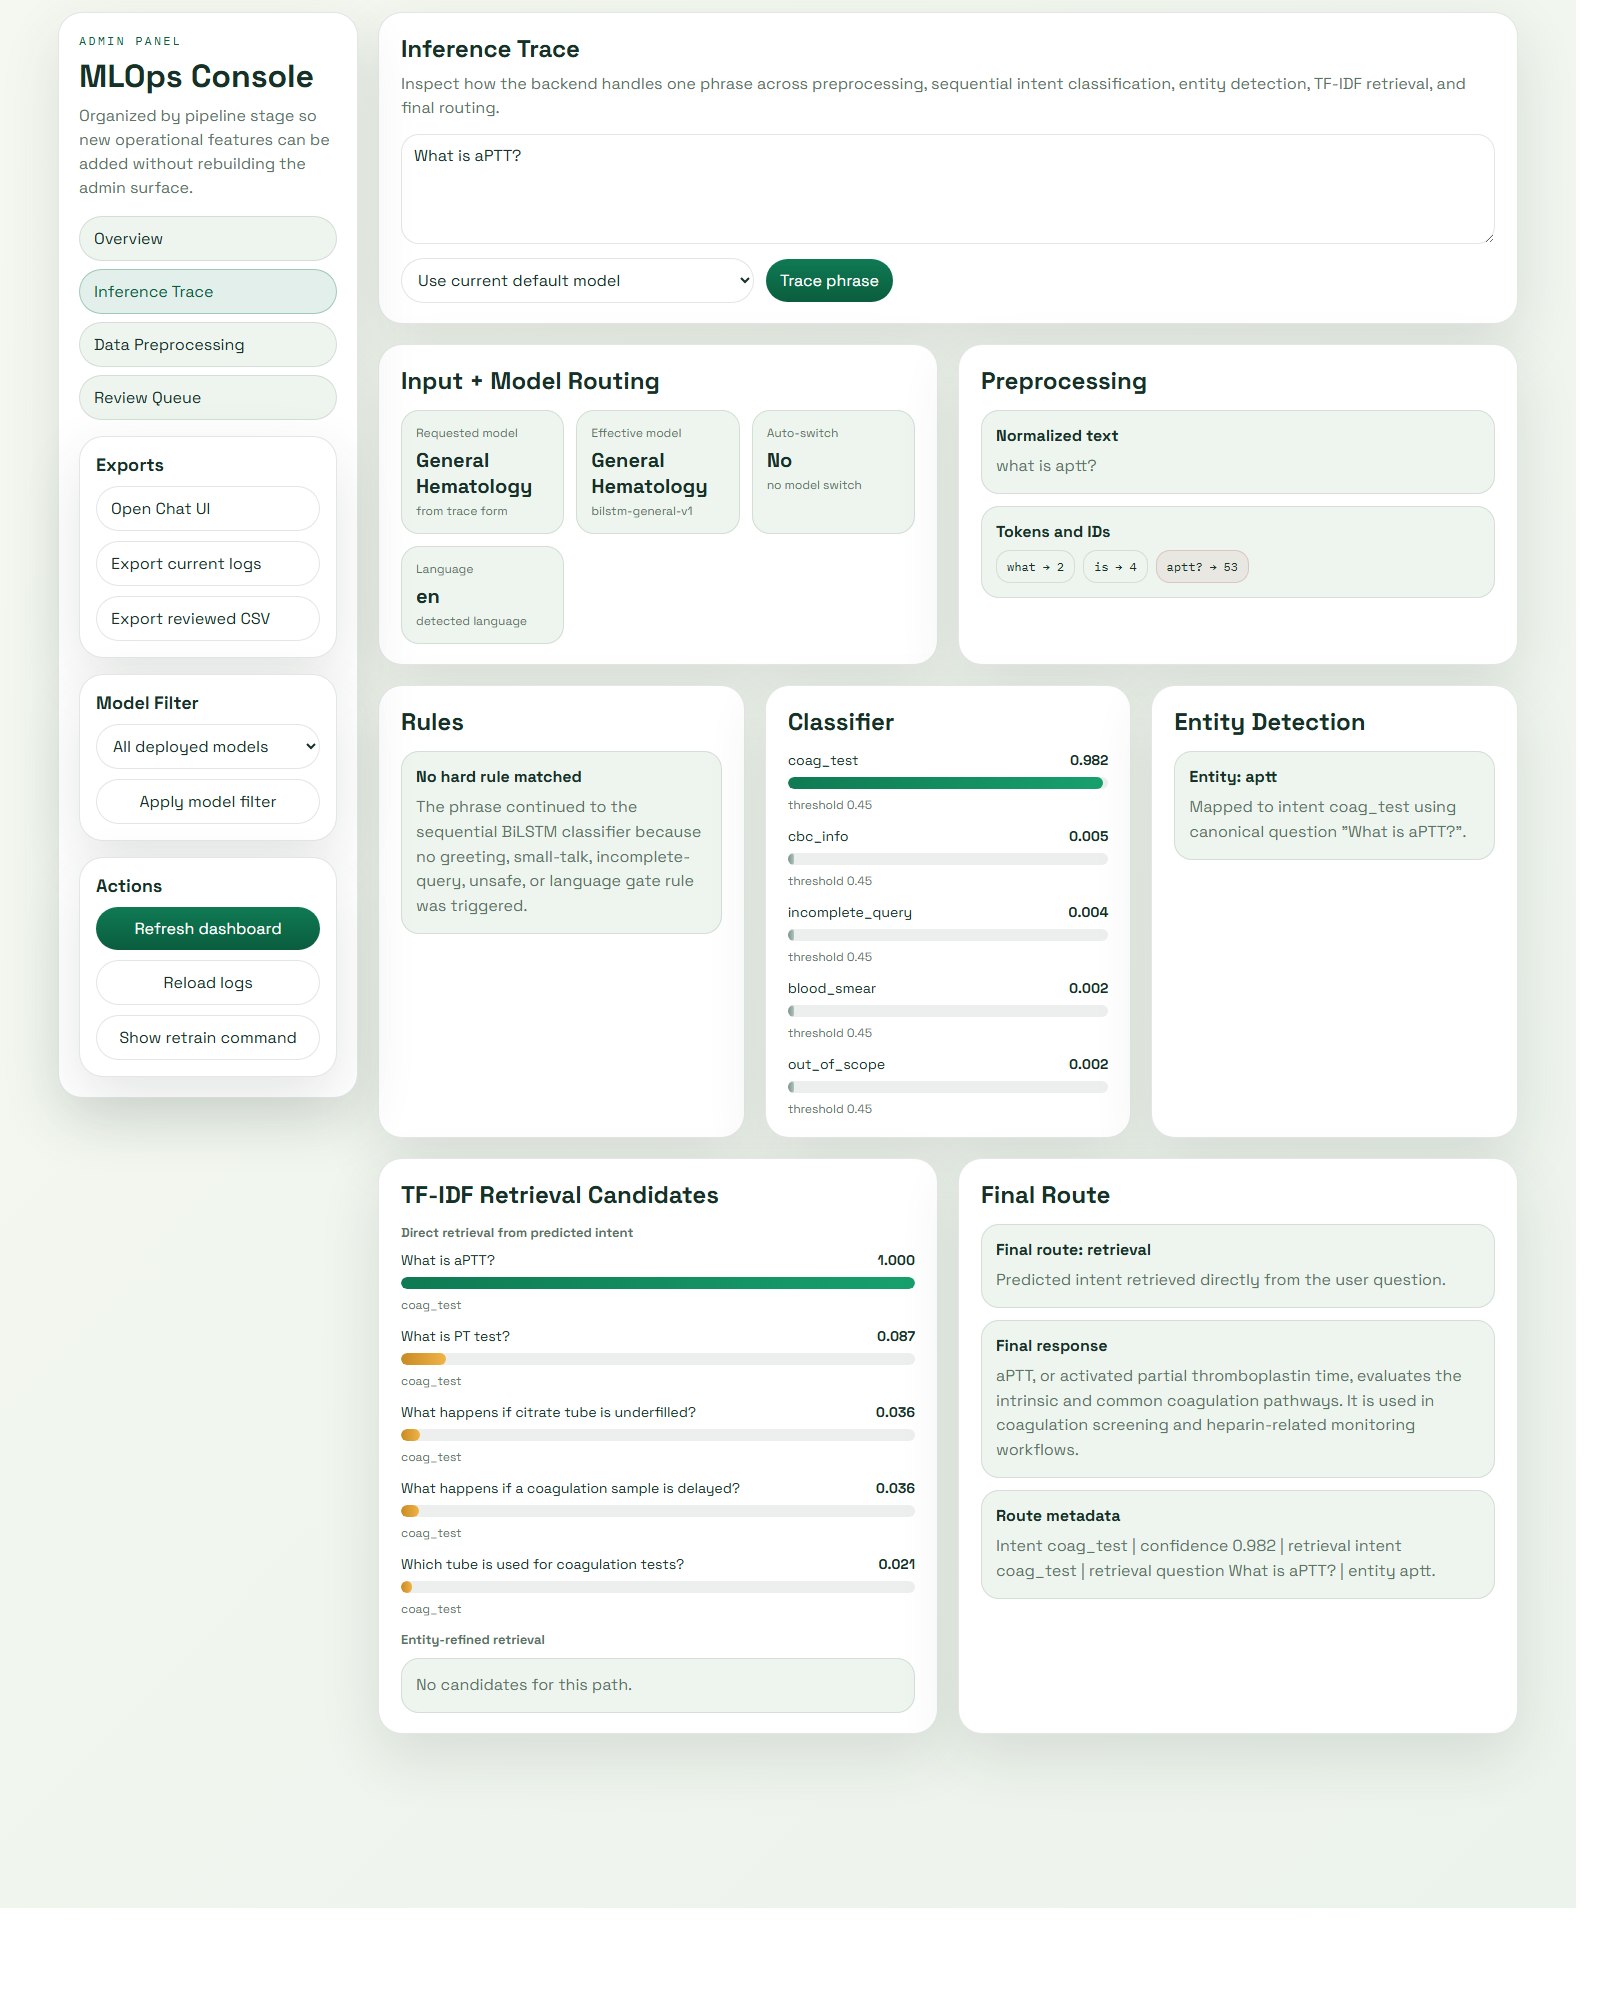
\includegraphics[width=0.88\linewidth]{figures/admin_trace.png}
    \caption{Inference trace view showing how a phrase was processed across the NLP pipeline.}
    \label{fig:admin-trace}
\end{figure}

The admin console provided evidence that the system was not merely trainable but operable. The overview displayed chat volume, average confidence, fallback rate, low-confidence rate, guardrail rate, retrieval rate, and auto-switch rate. The data preprocessing view exposed labelled sources, dataset footprints, version-relevant timestamps, and fixed split counts. The review queue supported log inspection and correction of misclassified phrases. The inference trace exposed how the backend handled an individual question.

The final browser UI also exposed a model-aware coverage panel so that the supported haematology topics of the \texttt{general} and \texttt{report} models were visible to the user. This reduced ambiguity around what each model was expected to do and aligned the interface more closely with the underlying architecture.

From an MLOps perspective, this was a major project strength. The system did not rely solely on offline metrics. Instead, it supported observation of live traffic, review of weak queries, export of reviewed phrases, and retraining from feedback. In practical terms, this meant the system could improve through usage rather than remaining a static demo.

\subsection{Advantages of the Implemented Approach}

Several advantages became clear during evaluation.

First, the sequential BiLSTM design remained computationally lightweight and practical for local deployment. Second, the retrieval-based response layer preserved answer control in a sensitive medical context. Third, the two-model architecture separated workflow support from report support while still allowing automatic switching for convenience. Fourth, the split-aware training and evaluation pipeline improved the credibility of reported metrics. Fifth, the admin console, PostgreSQL logging, and retraining workflow provided a meaningful MLOps foundation rarely present in student chatbot projects.

An additional advantage was interpretability at the system level. Although the BiLSTM itself was still a neural model, the surrounding pipeline made the overall decision process more transparent. Tokenisation, top intent probabilities, entity routing, and retrieval candidates could all be inspected.

\subsection{Limitations}

The project also had clear limitations.

The first limitation was dataset scale. Although 5,391 labelled utterances were substantial for a final-year project, they were still modest compared with industrial NLP datasets. The second limitation was class imbalance. The report dataset imbalance ratio rose because report-analysis phrases became much more common than several smaller support intents. The third limitation was language coverage. Only English was supported. The fourth limitation was that entity detection and report-value extraction remained rule-based, which was efficient and inspectable but not semantically complete. The fifth limitation was scope restriction: the system did not provide diagnosis, treatment recommendations, or unrestricted patient-specific report interpretation.

A further limitation concerned formal user evaluation. While the admin interface and conversation flow were developed carefully, no large-scale human-subject usability study was completed within the project timeline. Therefore, usability claims had to remain cautious and evidence-based rather than overstated.

\subsection{Critical Reflection}

The most important critical lesson was that chatbot quality did not depend solely on the classifier. Several development issues initially appeared to be model failures but were later shown to be retrieval or routing problems. For example, a correctly predicted \texttt{sample\_collection} intent could still return a generic CBC response if broad entity routing was allowed to override operational scope. This reinforced the importance of evaluating the complete pipeline rather than treating the model as the only meaningful component.

A second lesson was that production-style machine learning requires explicit metadata, version awareness, and repeatable data handling. Once fixed splits, review-driven retraining, and monitoring had been added, the project became much stronger academically and technically. Those features did not move the system away from sequential modelling or retrieval-based generation; they made that architecture maintainable.


\section{Conclusions and Further Work}
\label{sec:conclusion}
The project set out to design and develop a hybrid chatbot for medical haematology using sequential models for intent classification and retrieval-based response generation. That aim was achieved. A substantial artefact was implemented that integrated BiLSTM classifiers, curated retrieval, safety rules, model switching, PostgreSQL logging, a browser UI, an admin monitoring console, a retraining workflow, and split-aware evaluation.

From a research perspective, the project demonstrated that sequential models remained appropriate for bounded intent-classification tasks when the system scope was clear and the surrounding data and retrieval infrastructure was strong. From an engineering perspective, the project demonstrated that a small-scale MLOps implementation could still include important lifecycle concepts such as data staging, version-aware artefacts, train-validation-test separation, automated testing, monitoring, and feedback-based retraining.

The final results were credible rather than inflated. Test accuracy remained close to or above 0.90 across both model profiles, macro F1 remained above 0.86, and the full automated test suite passed with 52 tests. At the same time, the project acknowledged its constraints: moderate dataset size, English-only operation, rule-based entity refinement, and the deliberate exclusion of diagnosis and unrestricted patient-specific interpretation.

Several directions for further work were identified. Additional real user phrasing should be collected to reduce reliance on synthetic paraphrases and to improve communication-class robustness. More report-oriented entity coverage could be added, especially for fine-grained blood count flags, morphology terms, unit-aware parsing, and richer multi-parameter report interpretation. Formal usability testing with laboratory users should be conducted using structured instruments. The retrieval layer could be expanded with richer ranking and explanation support. Finally, multilingual support and document-grounded report assistance could be investigated, provided that the safety boundary remained explicit.

Overall, the project satisfied the goals of a final-year software and machine learning dissertation. It combined theoretical grounding, technical implementation, operational evaluation, and critical reflection into one coherent body of work.


\nocite{denecke2022,graves2005,hochreiter1997,kreuzberger2023,milneives2020,salton1988,sculley2015,tudorcar2020}
\printbibliography[title={References}]

\end{document}
